\documentclass[num-refs]{wiley-article}
% Written for the Overleaf "Wiley Journal Template" (class wiley-article.cls).
\usepackage{tabularx}
\usepackage{amsmath}
\renewcommand{\topfraction}{0.9}
\renewcommand{\bottomfraction}{0.8}
\renewcommand{\textfraction}{0.08}
\renewcommand{\floatpagefraction}{0.85}
\setcounter{topnumber}{3}
\setcounter{totalnumber}{4}

\papertype{Original Article}
\paperfield{Journal Section}

\title{Perplexity-Guided Joint Compression of Large Language Models for Resource-Constrained Inference}

\author[1]{Mohammad Adel Lootah}
\author[1\authfn{1}]{Sajid Gul Khawaja}
\affil[1]{College of Engineering, Abu Dhabi University, Abu Dhabi, United Arab Emirates}

\corraddress{Sajid Gul Khawaja, PhD, College of Engineering, Abu Dhabi University, Abu Dhabi, United Arab Emirates}
\corremail{sajid.khawaja@adu.ac.ae}

\runningauthor{Lootah and Khawaja}

\begin{document}

\maketitle

\begin{abstract}
Large language models are expensive to run because their weights and their key--value (KV) cache must fit in GPU memory, and the speed of writing each token depends on how fast that memory can be read. Compressing a trained model lowers this cost, but most published methods use the same setting for every layer and are tested only in simulation, not in the engine that runs the model. This paper presents a framework that deals with both problems. A first stage measures how much the perplexity rises when each layer is skipped and uses this to write a plan for each layer. Published quantization, pruning and KV-cache methods are then run with the same setting for every layer and with the planned setting, using the same code. Every model is measured in Hugging Face Transformers, llama.cpp and vLLM, and a Bayesian search chooses the full pipeline under limits on perplexity and on the time per token. On TinyLlama (1.1 billion parameters), five of the 22 layers matter far more than the rest. Giving 8 bits to the layers that matter most lowers the perplexity of all eleven weight-quantization methods compared with 4 bits in every layer, for a file of 1.05~GB instead of 0.81~GB. Pruning does not make the model smaller or faster in the engines, and models with low-bit activations are 13 to 17 times slower than the uncompressed model in vLLM. The search gave two models that are about 60 percent smaller and 20 percent faster than the uncompressed model in vLLM (0.838~GB at 1.98~ms per token and 0.898~GB at 2.00~ms per token, against 2.200~GB at 2.54~ms). Their mean accuracy on four tasks is 11 and 21 percent lower.

\keywords{large language models, model compression, quantization, pruning, KV cache, perplexity, low-latency inference}
\end{abstract}

\section{Introduction}

Large language models (LLMs) are hard to run where memory and computing power are limited. The weights must fit in memory, and the speed of generating tokens is limited by how fast memory can be read \cite{lin2024awq}: at small batch sizes and sequence lengths, most of the time of each decoding step goes to loading the weights from memory \cite{pope2023efficiently}. In addition to the weights, the model keeps a key--value (KV) cache with the attention state of every earlier token. This cache is stored in GPU memory and grows in proportion to the sequence length and the batch size \cite{zhang2023h2o}.

Model compression reduces these costs. Quantization stores weights and activations in fewer bits \cite{frantar2023gptq,lin2024awq}, pruning removes weights \cite{sun2024wanda}, and KV-cache methods round or drop cached tokens \cite{zhang2023h2o,hooper2024kvquant}. Two problems remain. First, these methods are usually applied with the same setting in every layer, although the layers of an LLM differ in how sensitive they are to compression \cite{yuan2025asvd}. Second, they are judged mainly by the perplexity of a simulated model, a metric that has been described as fairly simple and widely questioned \cite{jaiswal2024compressing}, and the same compressed model is seldom tested in the inference engines that would run it.

This paper presents a framework that measures the sensitivity of each decoder layer directly, as the rise in perplexity when the layer is skipped, and turns this measurement into a plan for each layer: how many bits its weights and activations get, how much of it is pruned and how much of the KV cache it keeps. Published techniques then follow the plans, every resulting model is measured in real inference engines, and a search chooses the joint configuration under stated limits on perplexity and on decode latency (the time to generate one token). The contributions are:

\begin{itemize}
  \item A profiling stage based on perplexity that scores every decoder layer and writes per-layer plans for weight bits, activation bits, pruning ratios, KV-cache bits and the share of cached tokens to keep.
  \item A controlled comparison in which eleven weight-quantization techniques, three pruning techniques and six KV-cache techniques are each run with the same setting in every layer and with the measured plan, using the same code, data, seed and hardware.
  \item An evaluation in the engines: each model is exported to llama.cpp and vLLM, its real file size, memory and latency are measured, and the cases where simulated results change in the engines are reported.
  \item A multi-objective Bayesian search with limits over the joint pipeline of quantization, pruning and KV-cache compression, which produced models about 60 percent smaller and 20 percent faster than the uncompressed model in vLLM.
\end{itemize}

Section~\ref{sec:related} reviews related work. Section~\ref{sec:framework} describes the framework, Section~\ref{sec:method} the implementation and the experimental methodology, and Section~\ref{sec:results} the results. Section~\ref{sec:conclusion} concludes.

\section{Related Work}
\label{sec:related}

\textbf{Quantization.} Post-training quantization is the most studied family. GPTQ rounds the weights one column at a time and compensates the error with second-order information \cite{frantar2023gptq}, AWQ scales the most important weight channels, which it finds from the activations \cite{lin2024awq}, and SmoothQuant moves the quantization difficulty from the activations to the weights \cite{xiao2023smoothquant}. SpQR and SqueezeLLM treat outlier or sensitive weights separately \cite{dettmers2024spqr,kim2024squeezellm}, OmniQuant learns clipping and equivalent transformations \cite{shao2024omniquant}, QuaRot rotates the model to remove outliers before rounding weights, activations and the KV cache \cite{ashkboos2024quarot}, QuIP and QuIP\# target 2 to 4 bits with incoherence processing and lattice codebooks \cite{chee2023quip,tseng2024quipsharp}, and PB-LLM binarizes most weights \cite{shang2023pbllm}. These methods reduce the size strongly, but how much faster the model runs depends on whether the serving engine has kernels for low-bit weights.

\textbf{Pruning.} SparseGPT prunes very large models in one shot with approximate second-order information \cite{frantar2023sparsegpt}, and Wanda prunes by the product of weight magnitude and input activation, without updating the remaining weights \cite{sun2024wanda}. Structural methods such as SliceGPT delete rows and columns of the weight matrices \cite{ashkboos2024slicegpt}. Unstructured pruning lowers the number of parameters, but it makes the model faster only when the engine has sparse kernels, and the reduction is often reported without a measured latency.

\textbf{Joint methods and distillation.} DayPQ chooses pruning and quantization for each layer and designs the algorithm and the hardware together \cite{xu2026daypq}. Such combined methods report some of the largest speedups, but on custom hardware, and the literature gives no clear rule for choosing between quantization only, pruning only and a combination. Knowledge distillation instead trains a smaller dense model, as in MiniLLM \cite{gu2024minillm}; it needs a teacher model and training, which is outside the methods used here.

\textbf{KV-cache compression.} H2O keeps the heavy-hitter tokens and drops the rest \cite{zhang2023h2o}, SnapKV selects the positions that an observation window attends to \cite{li2024snapkv}, KVQuant quantizes the cache below 4 bits \cite{hooper2024kvquant}, and InfiniGen predicts which tokens to fetch from an offloaded cache \cite{lee2024infinigen}.

\textbf{Evaluation metrics and tools.} Compressed LLMs are judged mainly by perplexity, and a comprehensive evaluation of quantized LLMs has been called essential for choosing a method \cite{li2024evaluating}. For deployment, Hugging Face Transformers provides the reference implementation of the models \cite{wolf2020transformers}; llama.cpp is a C/C++ engine without dependencies, with integer quantization from 1.5 to 8 bits and its own GGUF file format \cite{ggml2025llamacpp,ggml2025gguf}; and vLLM is a serving system that stores the KV cache in small blocks that do not have to sit next to each other in memory, which removes almost all wasted cache memory \cite{kwon2023vllm}. Each engine converts the weights into its own quantization types, so the quality and speed measured in an engine can differ from the simulated values.

Table~\ref{tab:related} compares representative studies. It shows three gaps. The methods are rarely compared under the same conditions. Their reported gains depend on particular kernels or hardware, so the same model is seldom measured in more than one engine. And the compression settings are rarely chosen for each layer from a stated requirement on latency, memory or quality. The framework of the next section addresses these three gaps on one model.

\begin{table}[tp]
\caption{Representative compression studies. Results are those reported by the cited papers.}
\label{tab:related}
\scriptsize
\renewcommand{\arraystretch}{1.15}
\begin{tabularx}{\textwidth}{>{\raggedright\arraybackslash}p{2.6cm}>{\raggedright\arraybackslash}p{2.9cm}>{\raggedright\arraybackslash}X>{\raggedright\arraybackslash}p{3.3cm}}
\hline
\textbf{Reference, year} & \textbf{Technique} & \textbf{Reported result} & \textbf{Deployment dependency or limitation} \\
\hline
GPTQ \cite{frantar2023gptq}, 2023 & One-shot weight quantization & 3 to 4 bits; about 3.25$\times$ speedup on an A100 & Low-bit kernels \\
AWQ \cite{lin2024awq}, 2024 & Activation-aware weight scaling & 3- and 4-bit weights with accuracy preserved & Low-bit kernels \\
QuaRot \cite{ashkboos2024quarot}, 2024 & Hadamard rotation & 4-bit weights, activations and KV cache; about 99\% zero-shot retention & Rotated kernels \\
SparseGPT \cite{frantar2023sparsegpt}, 2023 & One-shot unstructured pruning & At least 50\% sparsity on models of 175 billion parameters & Sparse kernels needed for speedup \\
Wanda \cite{sun2024wanda}, 2024 & Magnitude-times-activation pruning & Effective pruning without weight updates & Sparse kernels needed for speedup \\
DayPQ \cite{xu2026daypq}, 2026 & Layer-wise pruning and quantization & Up to 3.44$\times$ speedup; under 1\% accuracy loss & Custom accelerator \\
MiniLLM \cite{gu2024minillm}, 2024 & Distillation for generative models & Students of 120 million to 13 billion parameters & Needs teacher and training \\
H2O \cite{zhang2023h2o}, 2023 & Heavy-hitter KV eviction & About 20\% of tokens kept; up to 29$\times$ throughput & Accuracy risk when attention shifts \\
KVQuant \cite{hooper2024kvquant}, 2024 & Sub-4-bit KV quantization & Under 0.1 perplexity loss at 3 bits & Custom CUDA kernels \\
InfiniGen \cite{lee2024infinigen}, 2024 & Speculative KV prefetch & Up to 3.0$\times$ over earlier KV-cache methods & Offloading architecture \\
\hline
\end{tabularx}
\end{table}

\section{Proposed Framework}
\label{sec:framework}

The framework separates two questions. \emph{Where} to compress (which layers keep more bits, which layers are pruned and how much of the cache each layer keeps) is decided once from a perplexity measurement and written into per-layer plans. \emph{How} to compress (which published technique does the rounding or the pruning) is decided separately. Because the two are separate, every technique can be run twice with the same code: with the same setting in every layer, called \emph{Standard}, and with the measured plan, called \emph{Our method}.

\subsection{Framework Architecture}

Figure~\ref{fig:arch} shows the five stages. Stage~0 takes the 16-bit floating-point (FP16) TinyLlama model and calibration text and writes the plans. Stages~1, 2 and 3 quantize the model, prune it and compress its KV cache by following the plans. Stage~4 measures the result. A search sits on top: it proposes one technique for each of Stages~1 to 3 and the plan settings, receives the Stage~4 measurements, and then proposes the next configuration.

\begin{figure}[tp]
\centering
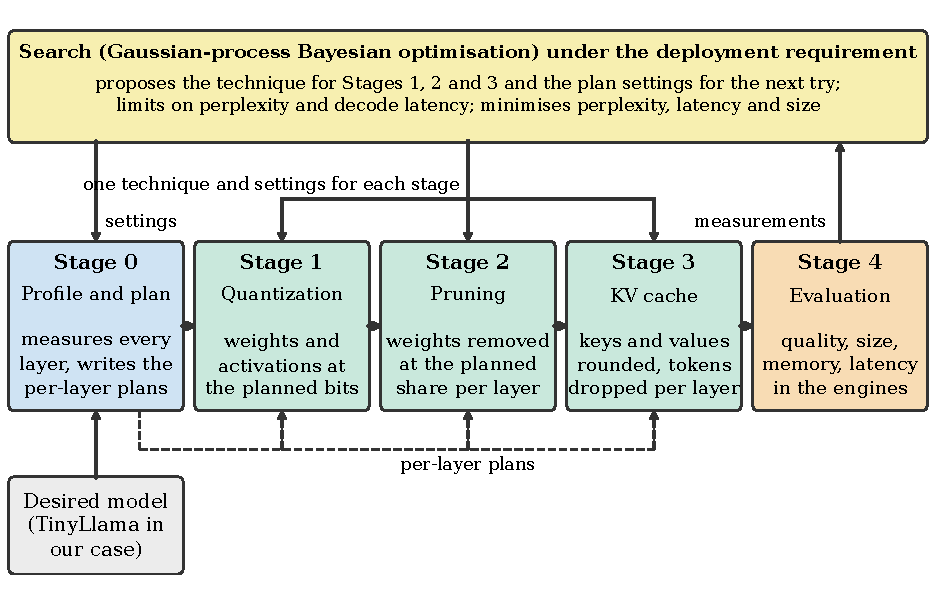
\includegraphics[width=0.75\textwidth]{Figures/ch4-framework-overview.pdf}
\caption{The framework. Stage~0 measures the model and writes per-layer plans; Stages~1 to 3 compress the model following the plans; Stage~4 evaluates the result. The search proposes the techniques and the plan settings and receives the measurements.}
\label{fig:arch}
\end{figure}

\subsection{Compression Modules}

Table~\ref{tab:modules} lists the techniques of each stage. Most are published methods that were re-implemented in a simpler form so that they can follow a per-layer plan. The stages can run one at a time on a fresh copy of the FP16 model, which shows the effect of a single stage, or one after another on the same model (quantize, then prune, then compress the KV cache), which is the joint pipeline used by the search. The quantization and pruning of Stages~1 and 2 are simulated in Hugging Face Transformers: the rounded values are written back into 16-bit tensors, and the model is then exported to the inference engines. The KV-cache techniques act inside the attention computation of the Hugging Face model.

\begin{table}[tp]
\caption{Compression modules of the framework.}
\label{tab:modules}
\small
\renewcommand{\arraystretch}{1.15}
\begin{tabularx}{\textwidth}{>{\raggedright\arraybackslash}p{2.4cm}>{\raggedright\arraybackslash}X>{\raggedright\arraybackslash}p{3.6cm}}
\hline
\textbf{Stage} & \textbf{Techniques} & \textbf{Standard setting} \\
\hline
1: quantization & Weights: round-to-nearest, GPTQ \cite{frantar2023gptq}, AWQ \cite{lin2024awq}, OmniQuant \cite{shao2024omniquant}, SqueezeLLM \cite{kim2024squeezellm}, SpQR \cite{dettmers2024spqr}, EfficientQAT \cite{chen2025efficientqat}, QuIP \cite{chee2023quip}, QuIP\# \cite{tseng2024quipsharp}, PB-LLM \cite{shang2023pbllm}, bitsandbytes storage. Activations: round-to-nearest, SmoothQuant \cite{xiao2023smoothquant} & 4-bit weights in every layer; 8-bit activations in every layer \\
2: pruning & Unstructured (Wanda criterion \cite{sun2024wanda}); structured removal of feed-forward channels; low-rank factorization (activation-aware SVD \cite{yuan2025asvd}) & The same pruning level in every layer \\
3: KV cache & Rounding: round-to-nearest, QuaRot \cite{ashkboos2024quarot}, KVQuant \cite{hooper2024kvquant}. Eviction: H2O \cite{zhang2023h2o}, SnapKV \cite{li2024snapkv}, InfiniGen \cite{lee2024infinigen} & 4-bit keys and values, all tokens kept; or 20\% of tokens kept at 16 bits \\
\hline
\end{tabularx}
\end{table}

\subsection{Perplexity-Guided Quality Assessment}

Quality is measured by perplexity. For a text of $N$ tokens,
\begin{equation}
  \mathrm{PPL} = \exp\left( -\frac{1}{N} \sum_{t=1}^{N} \log p(x_t \mid x_{<t}) \right),
  \label{eq:ppl}
\end{equation}
so a lower value means that the model gives the text a higher probability. Perplexity is used in three places. First, it is the sensitivity score: each decoder layer $l$ is skipped in turn, and the rise in perplexity on the calibration text is recorded,
\begin{equation}
  r_l = \mathrm{PPL}_{\mathrm{calib}}(\text{model with layer } l \text{ skipped}) - \mathrm{PPL}_{\mathrm{calib}}(\text{model}),
  \label{eq:score}
\end{equation}
and the scores are converted to ranks $s_l \in [0, 1]$, with $s_l = 1$ for the most sensitive layer. Second, it is the quality measure of every compressed model. It is computed on a validation set, which is used for all decisions, and on a held-out set, which is only reported. Third, it is a limit of the search: a configuration is accepted only if its validation perplexity is at most a stated value.

The weight plan follows from the scores with a threshold $\tau$ and a pruning ratio $\rho$:
\begin{equation}
  (b_l,\; p_l) = \left\{
  \begin{array}{ll}
    (8,\; 0) & \text{if } s_l \geq \tau \quad \text{(protected layer)} \\
    (4,\; \rho) & \text{if } s_l < \tau \quad \text{(compressed layer)}
  \end{array}
  \right.
  \label{eq:plan}
\end{equation}
where $b_l$ is the number of bits and $p_l$ the pruning ratio of layer $l$. In addition, the five layers with the largest $r_l$ are never pruned. The activation plan and the KV-cache plan are measured in the same way: the activations, the cached keys or the cached values of one layer are rounded to each candidate number of bits, the rise in calibration perplexity is recorded, and bits are given first to the layers where they remove the most measured damage, within a budget of 6 bits on average for activations and 4 bits for the cache. Each layer also keeps the smallest share of past tokens that still covers 95 percent of its attention.

\subsection{Joint Optimization Strategy}

A configuration of the joint pipeline consists of one technique for each of Stages~1, 2 and 3 and of numeric settings: the threshold $\tau$ (0.5 by default in the single-stage experiments; the search picks it between 0.8 and 0.9), the pruning ratio $\rho$ (0 to 0.3), the calibration dataset and the number of calibration windows, the quantization group size and the SmoothQuant strength. A deployment requirement is a set of upper limits. The requirement used here is a validation perplexity of at most 11.5 and a vLLM decode latency of at most 2.5~ms per token. Within these limits the search makes up to three objectives as small as possible: validation perplexity, decode latency and model size. The optimizer is multi-objective Bayesian optimization with a Gaussian-process model. For each configuration, the optimizer is told how far it misses the limits; a configuration that meets them gets zero.

\subsection{Framework Execution Workflow}

Figure~\ref{fig:workflow} shows one search run. For each proposed configuration, Stage~0 makes the plans from the cached measurements, one model is built through Stages~1, 2 and 3 in sequence, and the model is measured in Hugging Face and in vLLM. Both are needed: Hugging Face is where the compression is applied, so it gives the perplexity of the model as it was built, while vLLM is the engine that serves the model, so it gives the real file size and decode latency, which the simulated model does not show. The objective values and the distance from the limits are returned to the optimizer. A combination that was already built in an earlier run is not built again; its logged measurements are reused. After the last try, the configuration that meets every limit and is best on the first objective is built again as the final model and evaluated in full, including task accuracy.

\begin{figure}[tp]
\centering
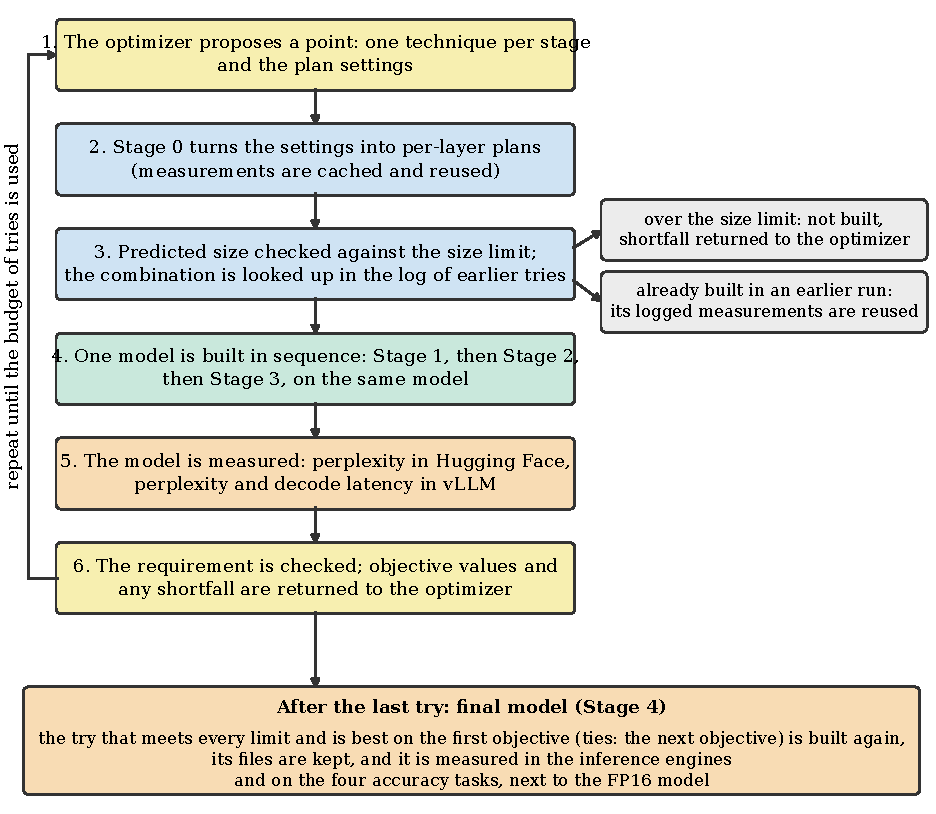
\includegraphics[width=0.5\textwidth]{Figures/ch4-search-loop.pdf}
\caption{Execution workflow of one search run. Each try builds one model through Stages~1, 2 and 3 in sequence and measures it; the final model is selected after the last try.}
\label{fig:workflow}
\end{figure}

\section{Implementation and Experimental Methodology}
\label{sec:method}

\subsection{Implementation}

The framework is written in Python with PyTorch and Hugging Face Transformers \cite{wolf2020transformers}. Each stage is a module with a common interface, so a technique is added by writing one function that receives the model and the plan. Results that take long to compute, such as the FP16 measurements and the Stage~0 profile, are stored in a cache whose key contains every setting that affects them. The search uses the Gaussian-process sampler of the Optuna library. llama.cpp is run through its conversion, benchmark and perplexity programs, with each decoder layer quantized at its planned number of bits in a GGUF file \cite{ggml2025gguf}. vLLM runs in its own Python environment and is started as a worker process; weight-only models are exported as a GPTQ-format checkpoint with per-layer bit widths, and models with rounded activations as a compressed-tensors checkpoint. An export to TensorRT-LLM \cite{nvidia2025tensorrtllm} is implemented but was not measured. The code has a suite of unit tests (481 passed and 3 skipped on the test GPU).

\subsection{Experimental Methodology}

\subsubsection{Models and Datasets}

All experiments use TinyLlama-1.1B-Chat-v1.0, a decoder-only model with 22 layers and 1.1 billion parameters that follows the architecture and tokenizer of Llama~2 \cite{zhang2024tinyllama}. The calibration data are 64 windows of 512 tokens from the training split of WikiText-2. The evaluation data are the test split of WikiText-2 cut into windows of 512 tokens; the first half of the windows is the validation set and the second half the held-out set. The search can also calibrate on C4 or on a sample of the Pile.

\subsubsection{Baseline Compression Methods}

There are two baselines. The first is the uncompressed FP16 model. The second is each technique with its Standard setting, which is the same in every layer (Table~\ref{tab:modules}). Our method is the same technique with the same code on the Stage~0 plan, at the default threshold $\tau = 0.5$ in the single-stage experiments. In the pruning experiments a third plan removes the same total number of weights as the Standard setting but places them by sensitivity, which gives a comparison at equal size.

\subsubsection{Evaluation Metrics}

Quality is the perplexity of Equation~\ref{eq:ppl} on the validation and held-out sets and, for the final models, the zero-shot accuracy on ARC-Easy, PIQA \cite{bisk2020piqa}, HellaSwag and WinoGrande \cite{sakaguchi2020winogrande}. Size is the file size of the exported model and the peak GPU memory. Speed is the decode latency per token at a batch size of one, measured with a prompt of 128 tokens and 64 generated tokens after 3 warm-up runs and averaged over 10 repeats, and the tokens per second reported by llama.cpp. llama.cpp scores only the second half of each window, so its perplexity can be compared only with other llama.cpp perplexities.

\subsubsection{Experimental Configuration}

Two GPUs were used: an NVIDIA A100 80~GB and an NVIDIA RTX~5070~Ti 16~GB. The quantization experiment ran on the RTX~5070~Ti and was measured in Hugging Face and llama.cpp. The pruning and KV-cache experiments and all searches ran on the A100, because vLLM (version 0.31.0) runs on Linux only. Pruning levels of 30 to 90 percent were tested. Every configuration was run with seed 0, and each search had a budget of 30 or 40 tries.

\section{Experimental Results and Discussion}
\label{sec:results}

The evaluation asks four questions: how much each technique compresses and what it costs in perplexity, with and without the plan; how the single stages compare with the joint pipeline; what the compression gives in memory and latency in real engines; and how much the results depend on the layers, the pruning level and the settings of the search. The FP16 reference has a perplexity of 10.18 on the validation set and 10.62 on the held-out set, a file of 2.20~GB, a vLLM decode latency of 2.54~ms per token and a mean accuracy of 0.625.

\subsection{Compression Performance and Quality Evaluation}

Figure~\ref{fig:dumbbell} compares the eleven weight techniques, measured on the RTX~5070~Ti. The Standard file is 0.81~GB (2.7 times smaller than FP16). The file of Our method, with 8 bits in the 11 protected layers, is 1.05~GB (2.1 times smaller). Our method has a lower perplexity than Standard for all eleven techniques, on both sets and in both engines (in llama.cpp with round-to-nearest, for example, 9.02 for Standard and 8.38 for Our method, with 8.12 for FP16). The gain is largest where 4 bits lose the most (PB-LLM, 11.70 to 10.48; round-to-nearest, 10.97 to 10.41) and smallest for the technique that is already close to FP16 (SpQR, 10.27 to 10.21). With the plan every technique is between 10.21 and 10.48, so the choice of technique matters much less than with the Standard setting; Figure~\ref{fig:gain} gives the gain of each technique in percent. The two are not compared at equal size: the plan wins back part of the quality lost at 4 bits (71 percent of the gap to FP16 for round-to-nearest) for 0.24~GB more.

\begin{figure}[tp]
\centering
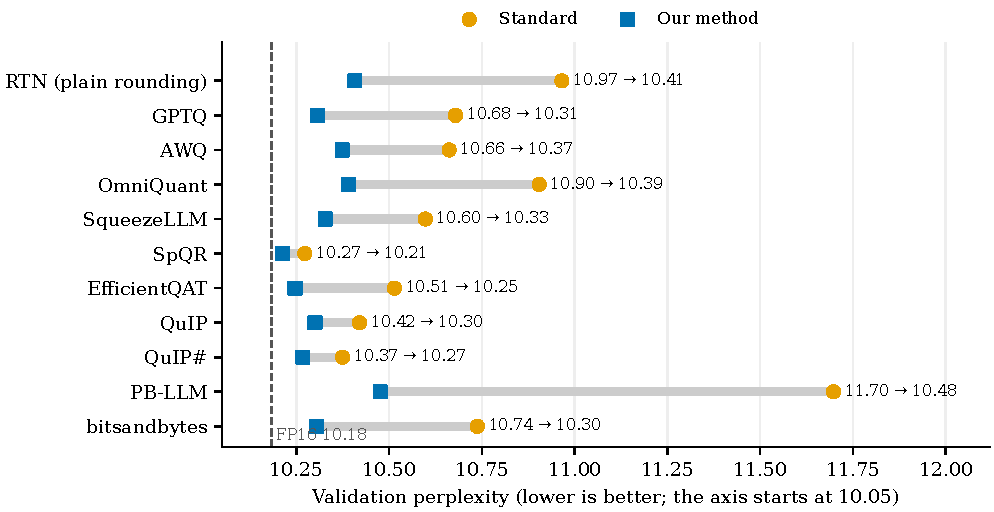
\includegraphics[width=0.62\textwidth]{Figures/ch5-quant-dumbbell.pdf}
\caption{Weight-only quantization: Hugging Face validation perplexity of each technique on the Standard plan (circle) and with Our method (square). Further left is better. The dashed line is the FP16 model.}
\label{fig:dumbbell}
\end{figure}

\begin{figure}[tp]
\centering
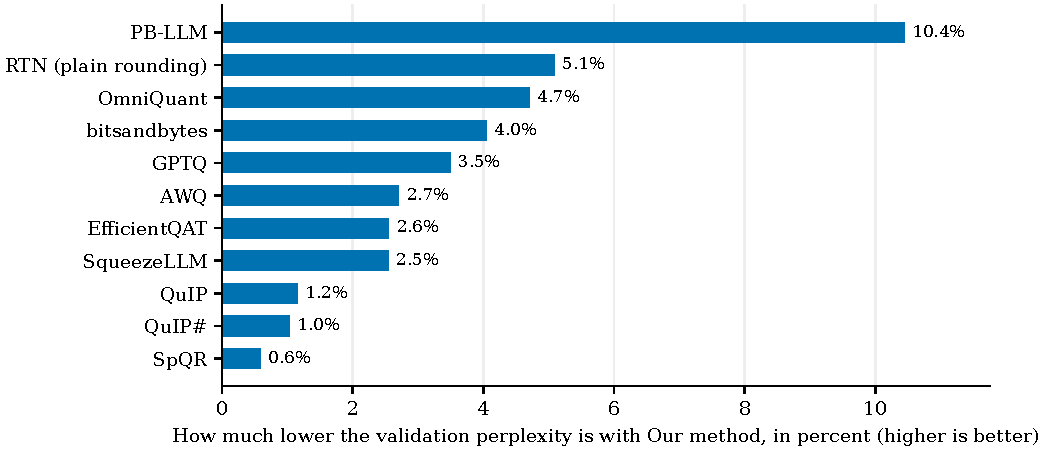
\includegraphics[width=0.58\textwidth]{Figures/ch5-quant-gain.pdf}
\caption{How much lower the validation perplexity of each weight technique is with Our method than on the Standard plan, in percent of the Standard value (a longer bar is a larger gain).}
\label{fig:gain}
\end{figure}

When the activations are rounded as well, the plan does not help in the same way. The Standard setting uses 8-bit activations in every layer, while the activation plan uses 6 bits on average. Our method was better than Standard for four of the twelve combined techniques and worse for eight (for SpQR, 10.28 for Standard and 10.64 for Our method). With 8-bit weights and activations in every layer, every technique is within 0.04 of the FP16 perplexity, with a file of 1.29~GB.

For the KV cache, measured in Hugging Face, the plan both rounds and drops tokens. It needs 3.2~MB for a context of 2{,}048 tokens, against 46.1~MB for FP16, 13.0~MB for 4-bit rounding in every layer and 9.2~MB for keeping 20 percent of the tokens in every layer. For five of the six techniques this smaller cache comes with a higher perplexity than the Standard setting; for example 11.68 against 10.25 for round-to-nearest rounding and 11.11 against 10.56 for SnapKV. With InfiniGen the plan is better on both counts (10.38 against 11.00).

\subsection{Comparative Evaluation}

\textbf{Single stages.} Of the three stages applied alone, quantization gives the best trade-off: a file 2.1 to 2.7 times smaller for a perplexity rise of 0.03 to 1.5. Pruning alone costs more quality and gives nothing back in the engines. At a level of 30 percent, unstructured pruning reaches 10.66 with the Standard setting and 10.37 with Our method, structured pruning 17.47 and 12.00, and the low-rank factorization 163 and 26.84, and the exported file stays at 2.20~GB in every case (Section~\ref{sec:resource}). KV-cache compression makes the cache smaller and leaves the model file unchanged.

\textbf{Joint pipeline.} Table~\ref{tab:finals} gives the final models of four searches over the joint pipeline. Figure~\ref{fig:finals} compares each final model with the FP16 model in vLLM, and Figure~\ref{fig:finals-size} shows the trade of quality against size. Under the two limits, the search for the lowest perplexity chose OmniQuant on the weights only (threshold 0.857, per-channel groups, 32 calibration windows of C4), unstructured pruning with a ratio of 0.082 and InfiniGen. When only weight-only quantization was allowed, the search chose round-to-nearest (threshold 0.800, which protects five layers; groups of 64; 128 windows of C4), no pruning and SnapKV. Both models are about 60 percent smaller and 20 percent faster than FP16 in vLLM. Two earlier searches, which had only the perplexity limit and size as the first objective, chose GPTQ with round-to-nearest activations and SqueezeLLM with SmoothQuant. These two models are just as small but 13.5 and 16.7 times slower than FP16 in vLLM, because vLLM runs models with rounded activations on slower kernels. The searched models use a higher threshold than the single-stage experiment (0.76 to 0.88 against 0.5), so fewer layers keep 8 bits: their vLLM files are 0.84 to 0.90~GB and their Hugging Face perplexity is 11.1 to 11.5, against 10.2 to 10.5 for Our method in Figure~\ref{fig:dumbbell}. In the two models within both limits the pruning ratio chosen by the search is zero or small: the search itself turns pruning nearly off.

\begin{figure}[tp]
\centering
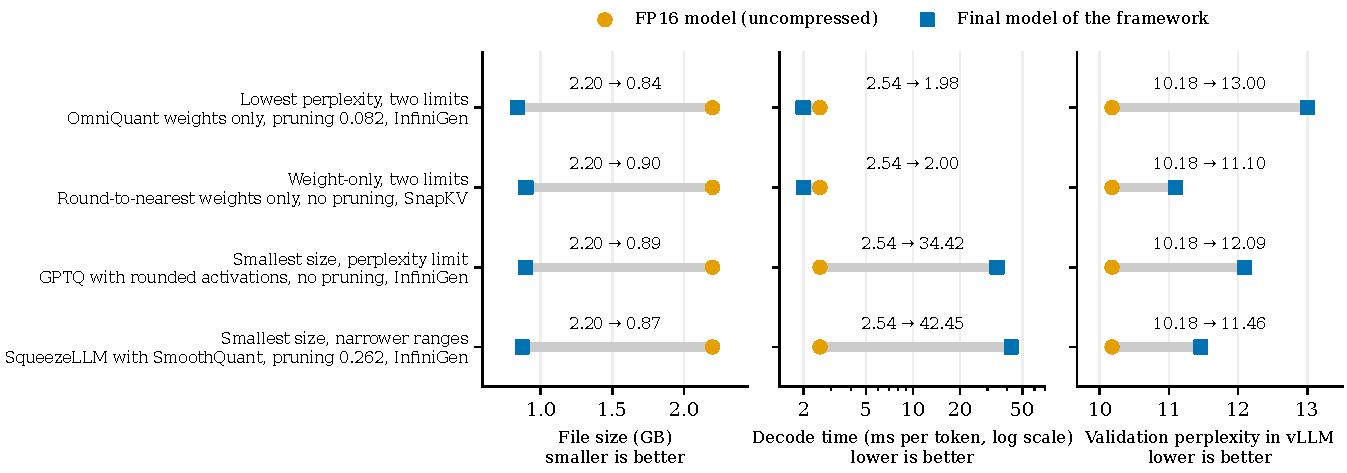
\includegraphics[width=0.95\textwidth]{Figures/ch5-finals-dumbbell.pdf}
\caption{The full framework: each final model (square) against the FP16 model (circle), measured in vLLM. Each row names the search and the quantization, pruning and KV-cache settings of its final model; the KV-cache step runs only in Hugging Face. Further left is better in all three panels.}
\label{fig:finals}
\end{figure}

\begin{figure}[tp]
\centering
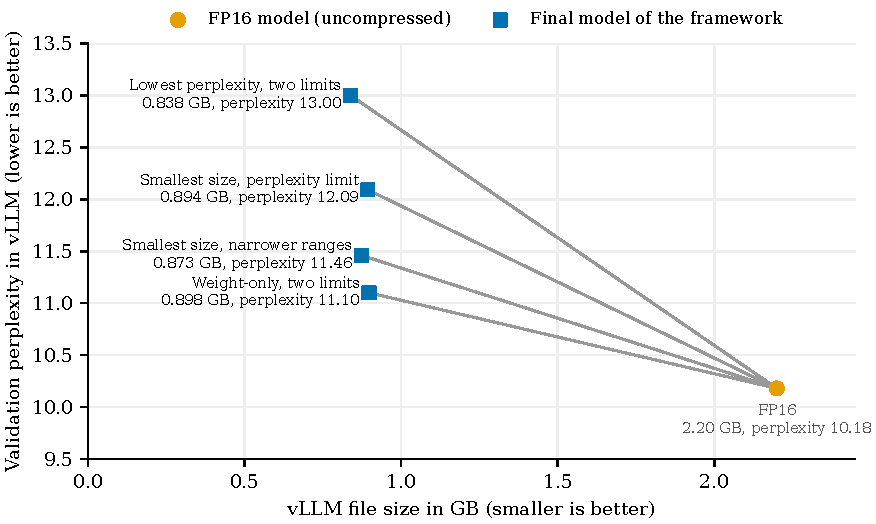
\includegraphics[width=0.6\textwidth]{Figures/ch5-finals-size.pdf}
\caption{Quality against size for the full framework. Each line joins the FP16 model (circle) to one final model (square). Lower is better for perplexity and smaller is better for size.}
\label{fig:finals-size}
\end{figure}

\begin{table}[tp]
\caption{Final models of four searches over the joint pipeline, measured in vLLM on the A100. Perplexity is given on the validation set and on the held-out set. Lower is better for size, perplexity, latency and memory; higher is better for accuracy. HF: Hugging Face.}
\label{tab:finals}
\scriptsize
\renewcommand{\arraystretch}{1.15}
\begin{tabularx}{\textwidth}{>{\raggedright\arraybackslash}p{1.9cm}>{\raggedright\arraybackslash}p{1.6cm}>{\raggedright\arraybackslash}X>{\raggedright\arraybackslash}X>{\raggedright\arraybackslash}X>{\raggedright\arraybackslash}X}
\hline
 & \textbf{FP16} & \textbf{Lowest perplexity, two limits} & \textbf{Weight-only, two limits} & \textbf{Smallest size, perplexity limit} & \textbf{Smallest size, narrower ranges} \\
\hline
Quantization & none & OmniQuant, weights only; $\tau$ 0.857; per channel; C4, 32 windows & Round-to-nearest, weights only; $\tau$ 0.800; group 64; C4, 128 windows & GPTQ with round-to-nearest activations; $\tau$ 0.759; group 128; WikiText-2, 64 windows & SqueezeLLM with SmoothQuant (0.638); $\tau$ 0.876; group 32; Pile, 128 windows \\
Pruning & none & Unstructured, 0.082 & Unstructured, 0 & Unstructured, 0 & Unstructured, 0.262 \\
KV cache & none & InfiniGen & SnapKV & InfiniGen & InfiniGen \\
\hline
vLLM file (GB) & 2.200 & 0.838 & 0.898 & 0.894 & 0.873 \\
HF perplexity & 10.18 / 10.62 & 11.50 / 11.91 & 11.12 / 11.52 & 11.23 / 11.62 & 11.44 / 11.87 \\
vLLM perplexity & 10.18 / 10.62 & 13.00 / 13.41 & 11.10 / 11.54 & 12.09 / 12.52 & 11.46 / 11.89 \\
Decode (ms/token) & 2.54 & 1.98 & 2.00 & 34.42 & 42.45 \\
Peak memory (GB) & 3.77 & 2.40 & 2.45 & 2.46 & 2.44 \\
Mean accuracy & 0.625 & 0.556 & 0.495 & 0.538 & 0.539 \\
\hline
\end{tabularx}
\end{table}

\subsection{Resource Utilization and Inference Efficiency}
\label{sec:resource}

\textbf{Quantization.} In llama.cpp on the RTX~5070~Ti, the 4-bit models run at 624 to 655 tokens per second and the models of Our method at 532 to 559, against 324 for FP16. In vLLM on the A100, weight-only models need about 2.0~ms per token against 2.54~ms for FP16, and their peak GPU memory is 2.40 to 2.45~GB against 3.77~GB (Table~\ref{tab:finals}). Models with rounded activations need 33 to 43~ms per token.

\textbf{Pruning.} Pruned weights are stored as zeros. For all 60 pruned models the llama.cpp and vLLM files are 2.20~GB, the vLLM decode latency is between 2.51 and 2.55~ms per token and llama.cpp runs at 412 to 426 tokens per second (FP16: 421). Pruning gave no gain in size or latency in these engines.

\textbf{Simulation against engines.} In Hugging Face, where the compression is simulated, the weight-only models need 4.09 to 4.22~ms per token against 4.32~ms for FP16, so the simulation shows neither the size gain nor the speed gain. The quality stays the same when the weights are exported without being rounded again (the pruned models agree to within 0.05 percent between Hugging Face and vLLM) and can change when the export rounds them again: 11.50 in Hugging Face and 13.00 in vLLM for the OmniQuant model, but 11.12 and 11.10 for the round-to-nearest model.

\textbf{Computing cost.} The Stage~0 profile needs one pass over the calibration text for the unchanged model and one for each layer. This took 96~s on the RTX~5070~Ti and 121~s on the A100, and the profile is reused by every later run. In two searches for the smallest model, the Bayesian optimizer built 30 models in 245 and about 190 minutes. Compared with successive halving, it found a smaller acceptable model in the first search (0.924 against 0.939~GB) and eight acceptable models against none in the second. Successive halving built 129 and 130 models in 495 and about 500 minutes.

\subsection{Ablation and Sensitivity Analysis}

\textbf{Layer sensitivity.} Figure~\ref{fig:sens} shows the score of Equation~\ref{eq:score}. The calibration perplexity of the unchanged model is 14.12. Skipping layer~0 raises it by 1{,}176 and skipping layer~2 by 368; layers 7, 21 and 1 follow with 36.5, 23.6 and 11.6, and the other 17 layers are between 1.4 and 5.7. Most of the sensitivity lies in the first three layers, one middle layer and the last layer.

\begin{figure}[tp]
\centering
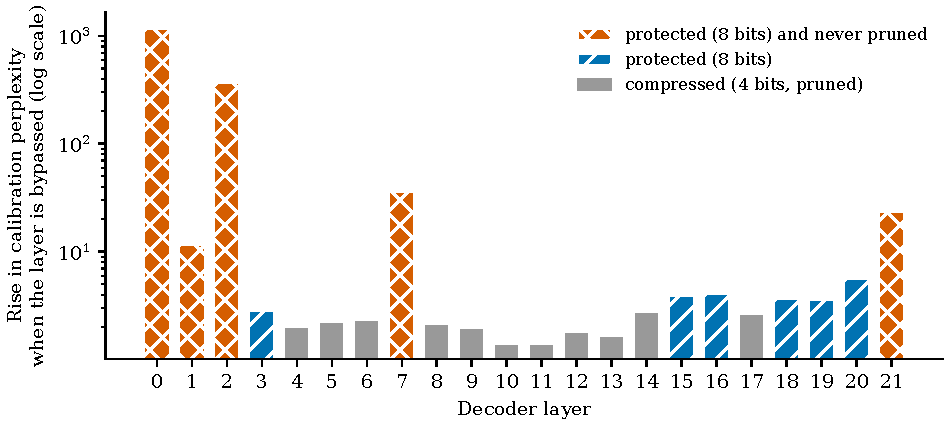
\includegraphics[width=0.68\textwidth]{Figures/ch5-sensitivity.pdf}
\caption{Sensitivity score of each decoder layer (log scale; a higher bar is a more sensitive layer) and the weight plan at the threshold $\tau = 0.5$.}
\label{fig:sens}
\end{figure}

\textbf{Pruning ratio and placement.} Figure~\ref{fig:prune} shows the perplexity against the pruning level. Our method leaves the protected layers unpruned and therefore removes about half as many weights (13 against 26 percent of all parameters at a level of 30 percent). It is better than Standard in all 20 comparisons; with unstructured pruning at 50 percent the perplexity is 11.51 against 14.12. The plan that removes the same total as Standard, but moves the pruning to the less sensitive layers, shows the effect of placement alone. It is worse than Standard in 19 of 20 comparisons (11.60 against 10.66 at 30 percent). The score therefore finds the layers to protect, but a layer that can be skipped with little damage cannot take a much larger share of the pruning.

\begin{figure}[tp]
\centering
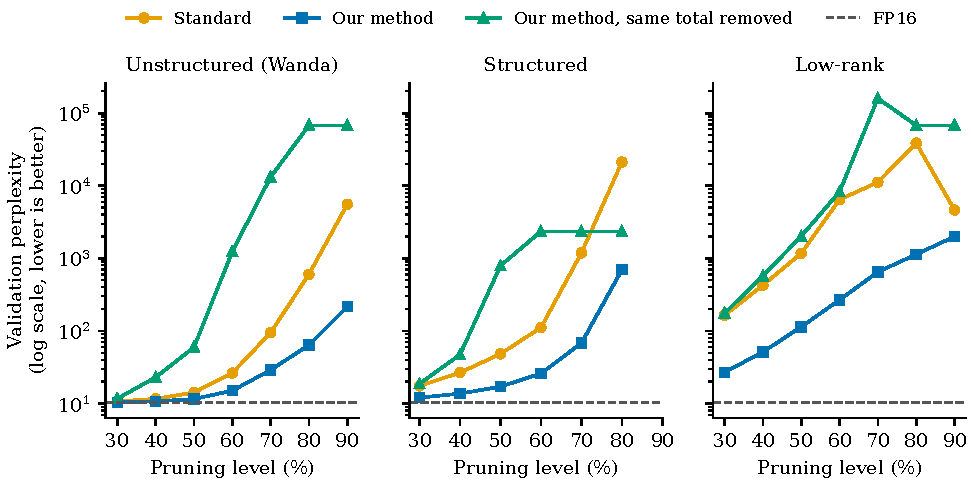
\includegraphics[width=0.72\textwidth]{Figures/ch5-pruning.pdf}
\caption{Hugging Face validation perplexity after pruning, against the pruning level (log scale; lower is better). The dashed line is the FP16 model.}
\label{fig:prune}
\end{figure}

\textbf{Limits and settings of the search.} Under the two limits, two of the 30 tries of the lowest-perplexity search and 17 of the 30 tries of the weight-only search met both limits. Lowering the perplexity limit to 11.0 left none, and lowering the latency limit to 2.0~ms left one, in effect the same model. With structured pruning as the only pruning technique, the closest try pruned nothing and reached 11.52.

\textbf{Where perplexity is judged.} Because the perplexity of an exported model can differ from its simulated perplexity, two further searches of 40 tries each checked the perplexity limit on the model as loaded in vLLM (Figure~\ref{fig:tries}). In each search, the 30 weight-only tries, all of which used OmniQuant, need 1.97 to 2.14~ms per token and have a vLLM perplexity of 12.97 or higher; the 10 tries with rounded activations need 33 to 43~ms, and one reaches 10.98. No try is within both limits. The round-to-nearest model of Table~\ref{tab:finals}, which was not proposed in these tries, is within both limits in vLLM (11.10 at 2.00~ms).

\begin{figure}[tp]
\centering
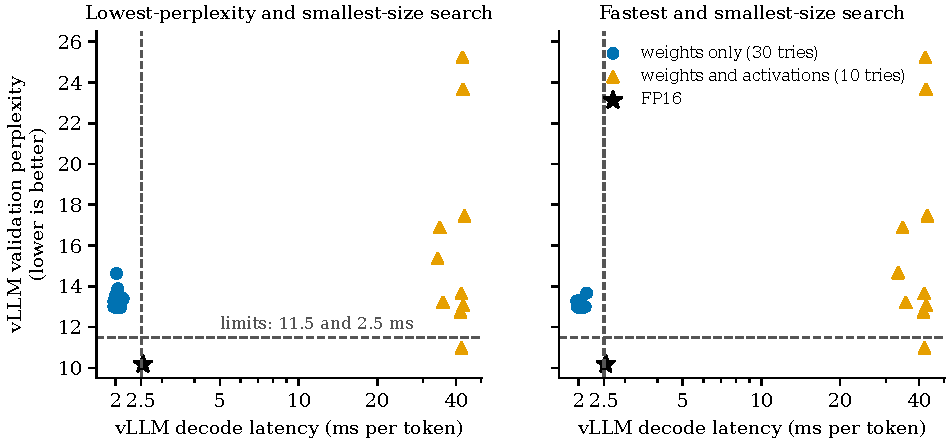
\includegraphics[width=0.68\textwidth]{Figures/ch5-search-tries.pdf}
\caption{All 40 tries of the two searches that judge perplexity in vLLM. Lower and further left is better. The dashed lines are the two limits; a try within both limits would lie in the lower left corner.}
\label{fig:tries}
\end{figure}

\subsection{Discussion and Limitations}

Three trade-offs stand out. First, a per-layer plan helps where the Standard setting has too few bits. It does not help where the plan spends fewer bits than the Standard setting (activations) or, in pruning, at equal size. Its practical value is that it brings a simple technique close to the best one: round-to-nearest with the plan (10.41) against SpQR with the Standard setting (10.27). Second, in the engines studied only weight-only quantization improves both size and latency; pruning improves neither, and low-bit activations reduce the size but not the latency in vLLM. Third, perplexity did not rank the final models by task accuracy: every final model lost 11 to 21 percent of the mean accuracy, and the model with the lowest perplexity lost the most. A requirement that is meant to protect accuracy needs an accuracy measurement among its limits.

The evidence has limits. The results are for one model of 1.1 billion parameters and one seed, on two GPUs and not on an edge device, so they may not carry over unchanged to other architectures, sizes or hardware. Most techniques are simplified re-implementations, and their numbers are not those of the original methods. Standard and Our method differ in size in the quantization experiment, and no comparison at equal size was made there. The KV-cache techniques run only in the Hugging Face model, their cache memory is computed from the plan, and they could not be exported. Finally, the number of tries of a search is small compared with the search space, and a search that found no acceptable configuration does not show that none exists.

\section{Conclusion and Future Work}
\label{sec:conclusion}

This paper presented a framework that measures the sensitivity of each decoder layer by perplexity, writes per-layer plans, applies published quantization, pruning and KV-cache techniques that follow the plans, measures every model in the engines that would run it, and searches the joint pipeline under limits on perplexity and decode latency. On TinyLlama, most of the sensitivity lies in five of the 22 layers. Protecting the sensitive layers improved the quality of every weight-quantization and pruning technique at a cost in size, but the plan gave no gain at equal size in pruning or with fewer activation bits. Quantization was the only stage that reduced size and latency in llama.cpp and vLLM, and simulated perplexity and latency changed in the engines. The search produced two models about 60 percent smaller and 20 percent faster than the uncompressed model: OmniQuant weight-only quantization with a pruning ratio of 0.082 and InfiniGen (0.838~GB, 1.98~ms per token), and round-to-nearest weight-only quantization with no pruning and SnapKV (0.898~GB, 2.00~ms per token).

Future work should repeat the study on larger models and with several seeds, compare the plan with the Standard setting at equal file size, round the weights directly to the values that the target engine can store, add task accuracy to the requirement of the search, measure engines that can store sparse weights, and build the KV-cache techniques into an engine and test them with longer contexts and larger batches.

\bibliography{references}

\end{document}
